\documentclass{article}

\usepackage{titlesec}
\usepackage{titling}
\usepackage[margin=1in]{geometry}
\usepackage{blindtext}
\usepackage{graphicx}

\titleformat{\section}
{\huge\bfseries}
{}
{0em}
{}[\titlerule]

\renewcommand{\maketitle}{
\begin{center}
	{\huge\bfseries
	\theauthor}
\end{center}
}

\newcommand\tab[1][2cm]{\hspace*{#1}}
\titlespacing{\subsection}{0em}{0.5em}{1em}

\begin{document}
\author{Shivang Patel}\date{}
\maketitle

\hrule
\vspace{10pt}

\begin{minipage}{.4\textwidth}
Plot No. 206/D-17,\\ Sarthak Co-op Housing Society,\\ RSC-33, Gorai II,\\ Borivali (West),\\ Mumbai - 400 092,\\ Maharashtra
\end{minipage}
\begin{minipage}{.39\textwidth}
\textbf{Contact Details}:\\ +91-9769194425\\ 022-2869-9461\\
\textbf{e-mail id}:\\ shivang705@gmail.com\\ shivang.patel@spit.ac.in
\end{minipage}
\begin{minipage}{.4\textwidth}
	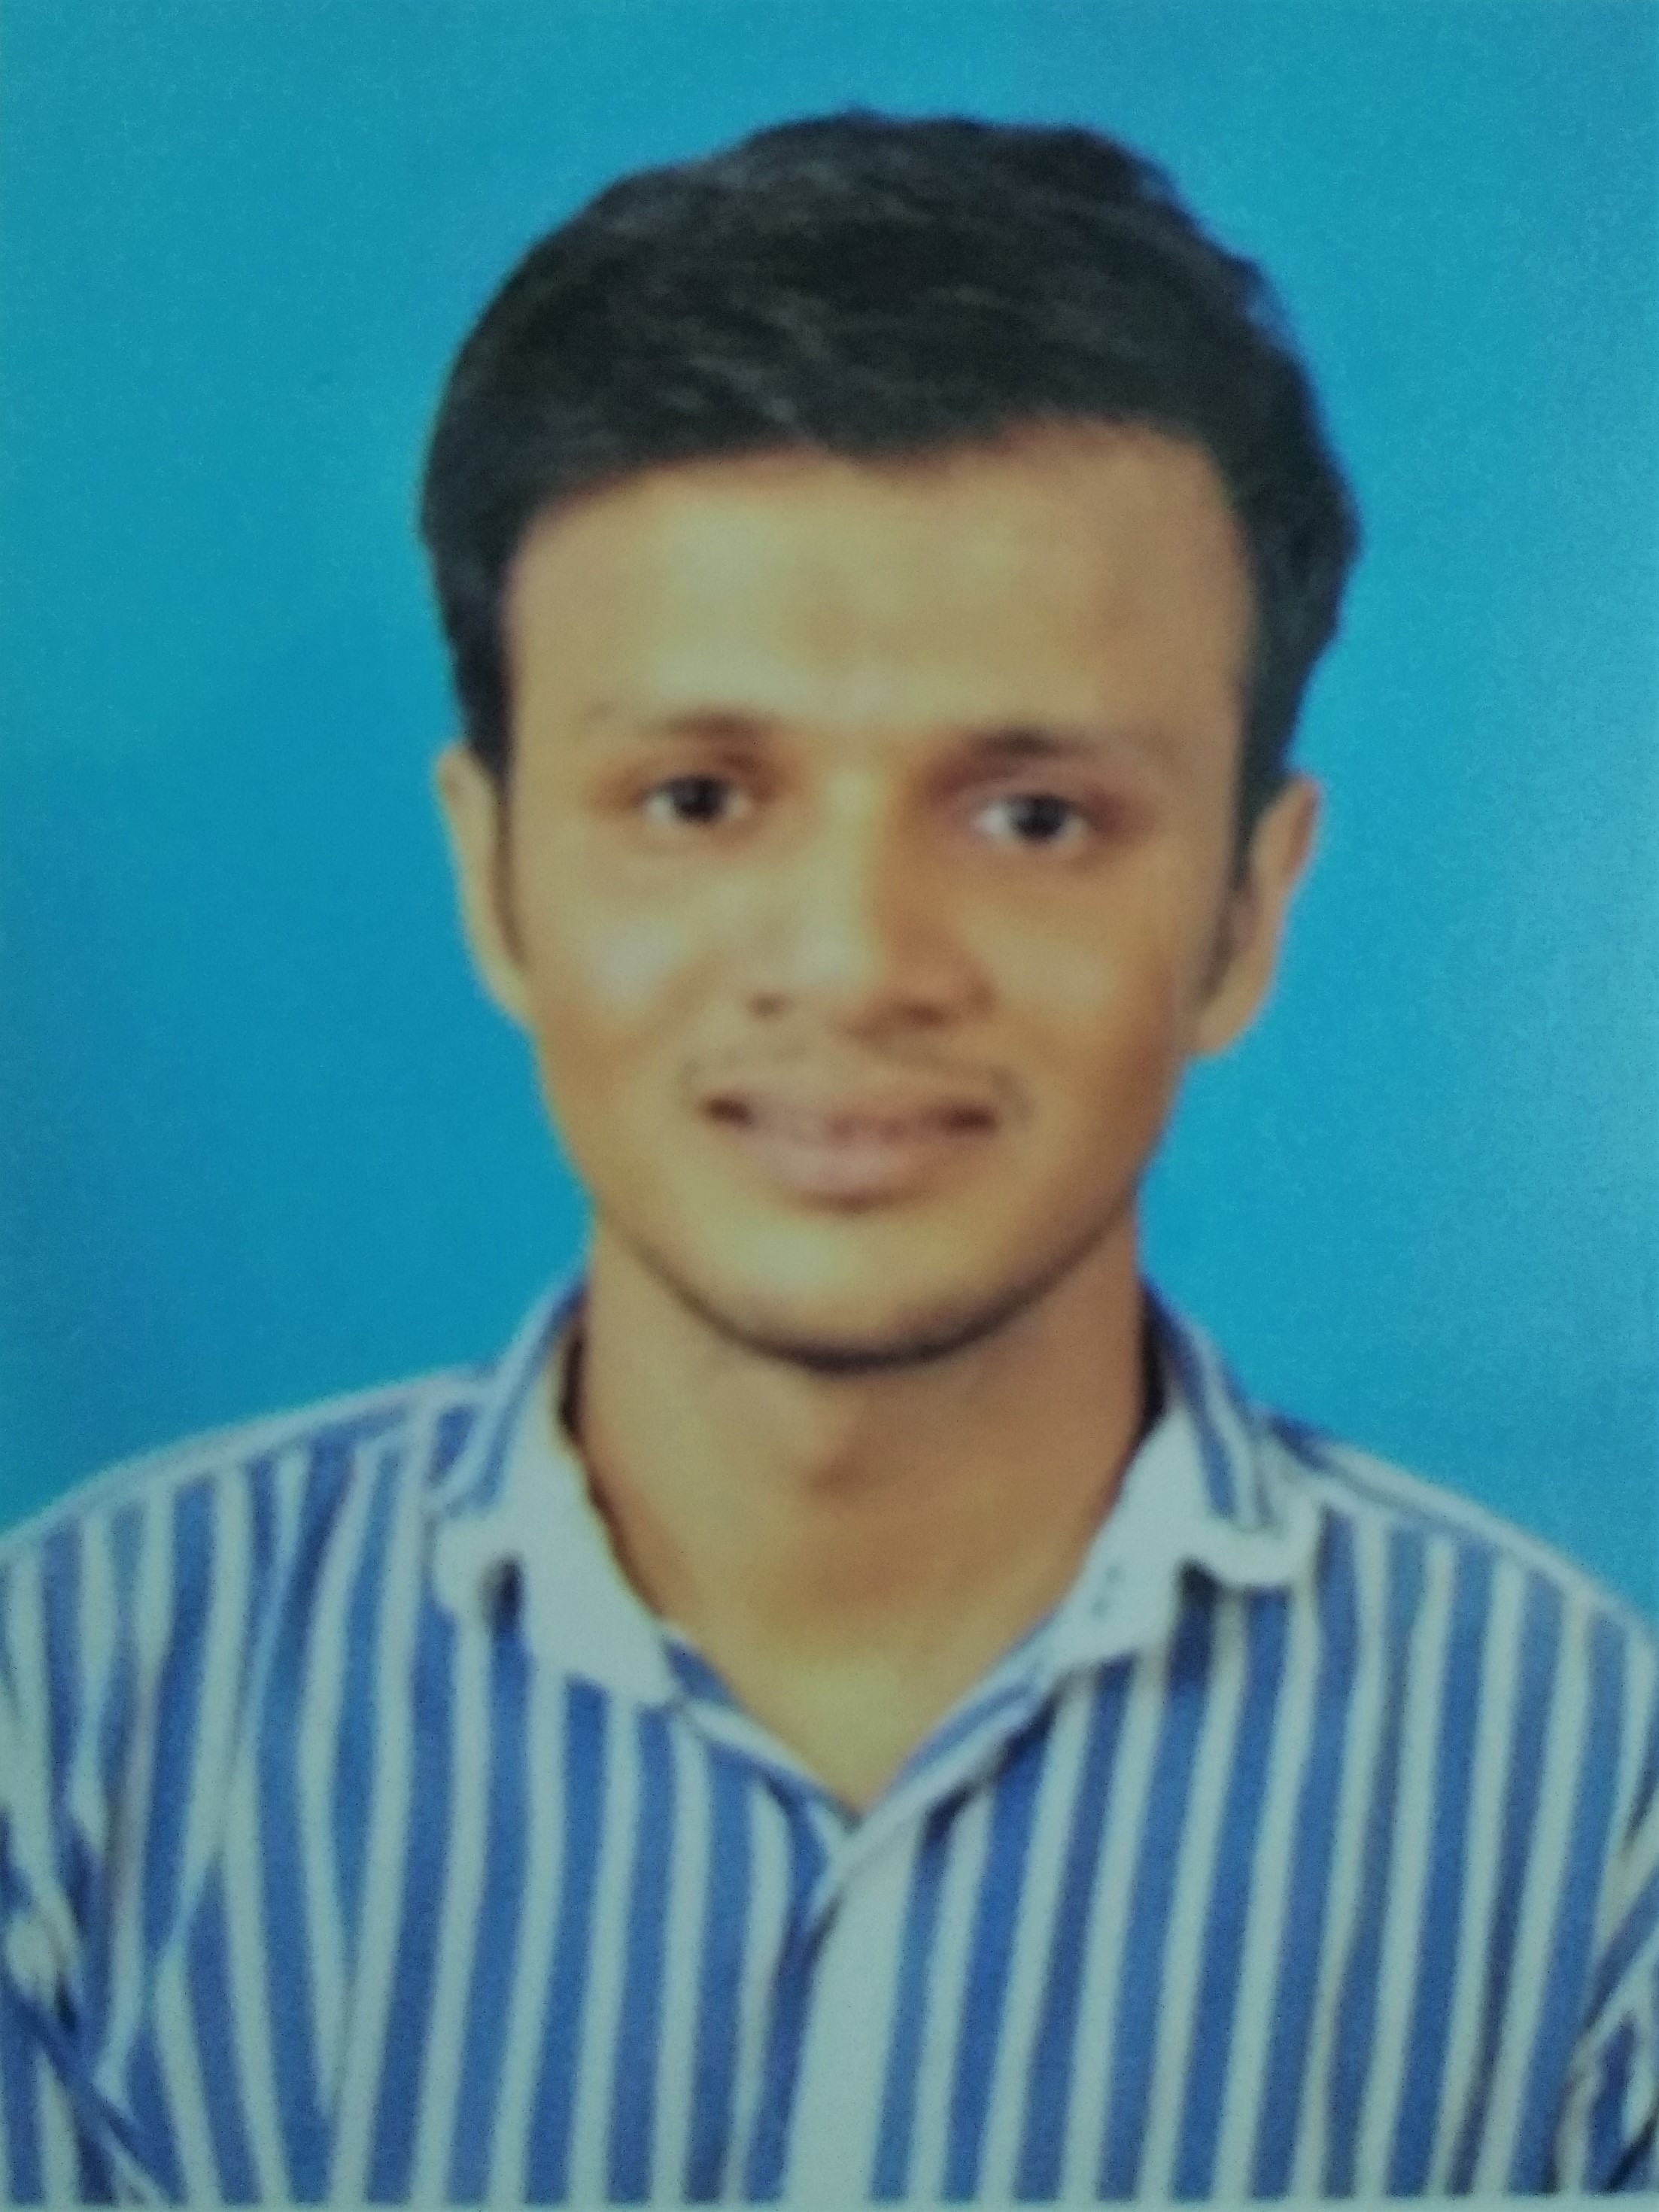
\includegraphics[scale=0.03]{myPhoto.jpg}
\end{minipage}

\section{Carrier Objective}
To work for an organization which provides me the opportunity to improve my skills and knowledge to growth along with the organization objective.
		
\section{Qualifications}
	\begin{center}
		\begin{tabular}{l l l l l }
			Degree & College/School & University & Passing Year & Pass \% \\ \hline \\
			SSC & St. Rocks High School & Maharashtra State Board & 2013 & 84.91\% \\ \\
			Diploma in  & Shri Bhagubhai & MSBTE & 2017 & 91.07\% \\ 
			Inustrial Electronics & Mafatlal Polytechnic
		\end{tabular}
	\end{center}

\section{Projects}
	\begin{enumerate}
		\item Controller Area Network (CAN) Communication.
		\item Serial Bootloader for Atmega and ARM controller using UART/USART.
		\item Flow Monitoring System.
		\item Timer Applications. 
		\item Counter Applications.
		\item Pick and Place Robot.
	\end{enumerate}

\section{Training \& Internship}
	\begin{itemize}
		\item Adavanced Control Data Machines (ifm electronic)
		\item Embedos Engineering LLP
	\end{itemize}

\section{Technical Skills}
	\begin{itemize}
		\item \textbf{Programming}: C, C++, C\#
		\item \textbf{Scripting}: Python, Visual Basics for Applications(VBA)
		\item \textbf{Markup}: {\LaTeX}, HTML, CSS
	\end{itemize}


\end{document}